\chapter{Introduction}
\label{cha:introduction}

\section{Motivation}
\label{sec:motivation}

Many of us have been struck by the inherent beauty of animals moving collectively; starlings gathering at dusk in huge numbers to perform the most mesmerising of ballets, the entire flock moving as if some fluid object; fish forming tight milling structures in defence against predation, changing direction in the blink of an eye and with a flash of silver. At different length scales, and in both the living and non-living domains, startling examples of collective behaviours have been observed.

\begin{figure}[!htbp]
	\centering
	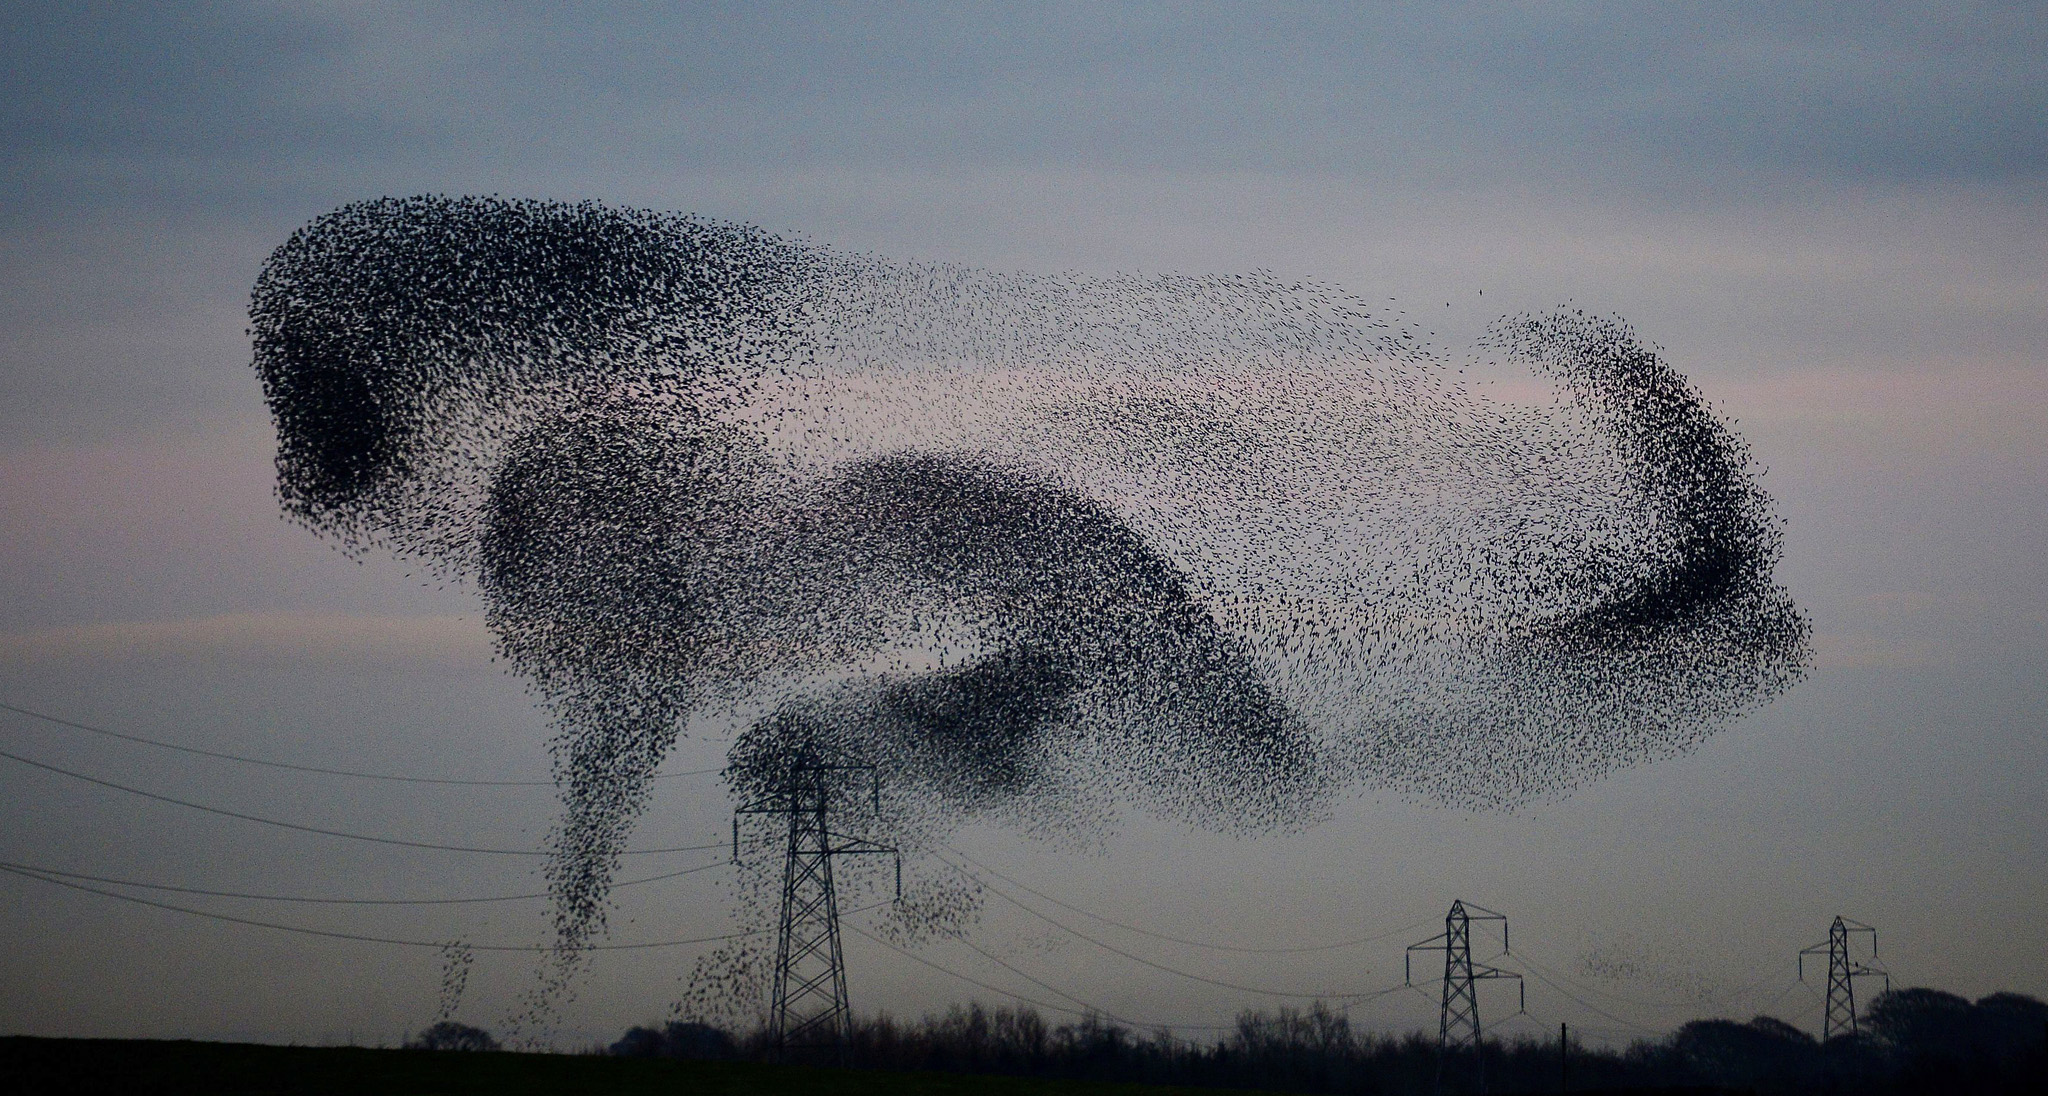
\includegraphics[width=\textwidth]{fig/murmuration.jpg}
	\caption{A particularly startling example of a starling murmuration, captured near Gretna in the Scotish Borders. Photograph: Owen Humphreys/PA.}
	\label{fig:murmuration}
\end{figure}

Over the years collective behaviour has become a thriving topic of multidisciplinary research, capturing the imaginations of physicists, biologists, mathematicians and statisticians. Our understanding has evolved significantly from early suggestions that collective behaviour results from thought-transference and telepathy between individuals \citep{selous31}. Though we can often explain why animal aggregations are evolutionary advantageous, little is in fact known about how these structures are formed in the first place.

Much work has been invested in developing theoretical models which seek to explain emergent behaviour by interactions at an individual level. Such models have shown that individual interactions are sufficient to produce group-level structures. Many different simulations, implementing disparate interaction rules, are able to produce behaviour reminiscent of real flocking systems. However, these models have largely only been verified with comparison to empirical observation at a qualitative level, and a thorough quantitative comparison between field data and theory has been lacking.

In recent years technological and methodological advances have made it possible to capture the movements of large groups of animal aggregates. With this data, it is only now that we are in a position to make a robust comparison between model predictions and real-world observations.

In this thesis we utilise real data to perform statistical inference on theoretical models. Our inference is made in a Bayesian framework. Bayesian inference allows the capture of uncertainty about fitted model parameters, flexible model structures and potential inclusion of expert information via the prior distribution. With this we seek to fit empirical data to a generalisation of a popular model from the literature.

\section{Biological Function}
\label{sec:biological_function}

Behaving as a group can bring many advantages to the individuals involved. One classically considered  benefit of aggregation is in the defence against predation. Shoaling fish groups have the ability to confuse predators, as predators have difficulty selecting an individual target \citep{landeau86}. As well as a confusion effect groups of individuals can be more vigilant than a single individual, allowing for the earlier detection of predators \citep{pitcher93}. Despite these advantages, groups may in fact attract predators \citep{wittenberger85}.

As well as providing defence against predation grouping can aid in foraging for food; collections of individuals are able to gather more information than lone individuals. In addition to foraging collective motion aids group navigation and migration \citep{simmons04}. For birds group navigation often brings an energetic advantage as individuals can work to form aerodynamically efficient shapes \citep{weimerskirch01}.

\section{Theoretical Models}
\label{sec:models}

Models of collective behaviour can largely be divided into two classes: Lagrangian and Eulerian. These descriptions are analogous to the models of fluid dynamics, where Lagrangian models consider the flow in terms of interactions of fluid parcels and Eulerian models consider the changing fluid properties at a given point in space and time. In the context of collective behaviour Lagrangian models simulate the movements of interactions and Eulerian models typically model the density of a group through space and time.

\subsection{Lagrangian Models}
\label{ssec:lagrangian_models}

So called agent-based models (ABMs), also referred to as Lagrangian models, have proven a useful tool in modelling collective behaviours. In these models the behaviour of an agent is modelled at the individual level. An agent's behaviour is determined by social interactions with neighbouring individuals. Examples of typical interactions include the desire to move in the same direction as neighbours (alignment, or orientation), the desire to avoid collisions (repulsion) and a desire to remain close to neighbours (attraction). Along with specifying social behaviours ABMs suggest methods by which agents identify neighbours to interact with. An individual may identify neighbours as; within a certain distance; positioned inside a field of vision or as one of a fixed number of closest agents.

In a pioneering paper, \citet{aoki82} developed an ABM to simulate the movements of schooling fish in two-dimensions. Here it was shown that collective behaviour can arise from simple interactions at an individual level and without the need of a leader. The model simulated zonal interactions in which the area around an individual is partitioned into zones of repulsion, alignment and attraction. The partitioning of space in this way is illustrated in Figure \ref{fig:zone_illustration}. As well as zonal interactions this model accounted for fish having incomplete fields of vision. Further models were also devised to simulate fish schools \citep{okubo86, huth92}.

\begin{figure}
	\centering
	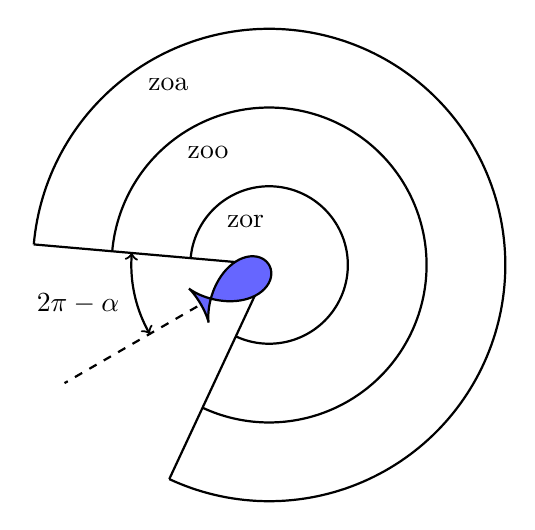
\begin{tikzpicture}[rotate=30]
		% draw zor
	   \draw [thick, domain=0:145, samples=100] plot ({cos(\x)}, {sin(\x)});
	   \draw [thick, domain=215:360, samples=100] plot ({cos(\x)}, {sin(\x)});
	   % draw zoo
	   \draw [thick, domain=0:145, samples=100] plot ({2*cos(\x)}, {2*sin(\x)});
	   \draw [thick, domain=215:360, samples=100] plot ({2*cos(\x)}, {2*sin(\x)});
	   %draw zoa
	   \draw [thick, domain=0:145, samples=100] plot ({3*cos(\x)}, {3*sin(\x)});
	   \draw [thick, domain=215:360, samples=100] plot ({3*cos(\x)}, {3*sin(\x)});
	   % close circle segments
	   \draw [thick] (0, 0) -- ({-3*sin(270-145)}, {-3*cos(270-145)});
	   \draw [thick] (0, 0) -- ({3*sin(145-200)}, {-3*cos(145-200)});
	   % line behind fish
	   \draw [thick, dashed] (0, 0) -- (-3, 0);
	   % make that sweet sweet fish curve
	   \draw [fill=blue!60!white, thick, domain=-200:200, samples=100] plot ({0.5*(cos(\x) - sin(\x)^2/1.41)-0.5}, {0.5*sin(\x)*cos(\x)});
	   \node [text width=1cm] at (0.25, 0.5) {zor};
	   \node [text width=1cm] at (0.25, 1.5) {zoo};
	   \node [text width=1cm] at (0.25, 2.5) {zoa};
	   % illustrate blind zone
	   \draw [<->, thick, domain=145:180, samples=100] plot ({1.75*cos(\x)}, {1.75*sin(\x)});
	   \node [text width=3cm] at (-1.5, 0.3) {$2\pi - \alpha$};
	\end{tikzpicture}
	\caption{An illustration of the area around an agent partitioned into multiple zones. zor: zone of repulsion, zoo: zone of orientation (or alignment), zoa: zone of attraction. The missing segment behind the agent represents the blind zone in which it cannot see.}
	\label{fig:zone_illustration}
\end{figure}

\citet{reynolds87} formulated a theoretical model, motivated by the production of computer animations, which described the movement of flocking birds in three-dimensional space. To produce more aesthetically pleasing animations, the software, ``Boids'', included sophistications such as banking during turns. This focus on developing simulations which produce elegant behaviour made rigorous scientific analysis difficult. Interestingly, Tim Burton's 1992 Batman Returns used a modified version of the Boids software to simulate animations of bat swarms and penguin flocks.

Motivated by research within statistical physics, \citet{vicsek95} introduced a simple two-dimensional model in which self-propelled particles move with a fixed absolute velocity and align with neighbours within an interaction zone. This model is commonly referred to as ``Vicsek Model" (VM), which we shall later use to formulate our ``Generalised Vicsek Model" (GVM). Despite its simplicity this model produces complex-behaviour resembling that of a real biological system. Vicsek et al. investigated the phase transition between ordered and disordered motion as the density of particles and noise in the system varied.

Later, models were developed to explore the movements of mammals and other vertebrate groups. \citet{couzin02} showed major group-level behavioural changes as minor changes in individual interaction rules were made. With small changes in the model parameters, groups transitioned from disordered, swarm like behaviour, to toroidal milling structures, to forming dynamic and highly parallel groups. Further research was made by \citet{couzin05} which investigated how leaders influence the motion of travelling groups. This work showed that only a small proportion of leaders are necessary to guide groups with a high degree of accuracy. Further results investigated how groups of individuals make collective decisions in the face of conflicting desires.

As a method for exploring collective behaviour, Lagrangian models are very appealing in their intuitiveness and in the ease of implementing explicit behavioural rules. Though for many years the simulation and exploration of these models was limited by computing power; modern computation allows for the simulations of large groups over many time steps. With these advances in computing, and a growing interest in the field, a significant proportion of the literature focuses on the analysis and exploration of agent-based models.

\subsection{Eulerian Models}
\label{ssec:eulerian_models}

Sometimes known as continuum models, Eulerian models are complementary to the Lagrangian method. This approach describes a group by the density of organisms at a point in space. Eulerian models are typically constructed of a set of partial differential equations which describe how density develops over time.

One such Eulerian approach by \citet{gueron93} modelled the movements of large groups of wildebeests. The predictions of the model were compared with aerial observations of migrating wildebeest in the Serengeti. The large-scale front patterns seen in the aerial photography were reproduced by the model.

Eulerian models have also been used to analyse vortex solutions \citep{topaz04} and stationary clump solutions \citep{topaz06}.

However, the Eulerian approach is limited. Most analyses are restricted to 1-dimension and the approach has not proven appropriate for modelling groups of low densities. With this in mind, and with the advantages of the Lagrangian approach, in this thesis we will concentrate entirely on modelling in the Lagrangian framework.

\section{Empirical Studies}
\label{sec:empirical_studies}

Real data of animal aggregations is essential to ensure that theoretical models are falsifiable. The emergence of a desired pattern from simulation is not sufficient evidence that a model is correctly capturing the interactions of individuals. This observation is further compounded by the understanding that models employing different local interactions can produce similar looking behaviour at the group level.

Thorough comparison between real data and model predictions have proven difficult largely because of the scarcity of appropriate data. The collection of suitable data can be a complicated and convoluted process. Taking observations in the field is technically demanding, requiring the precise calibration of sensitive measurement equipment, not to mention the additional difficulty of the typically three-dimensional nature of animal aggregations. Collecting data in a laboratory setting seems an obvious workaround - however this imposes restrictions on the types of behaviour which can be captured. A laboratory may be an appropriate environment to capture the movements of fish in a tank, but it certainly isn't appropriate to capture the movements flocking of birds. Despite the difficulties associated with collecting data, significant effort has been made to track the movements and dynamics of groups of individuals.

\begin{figure}
	\centering
	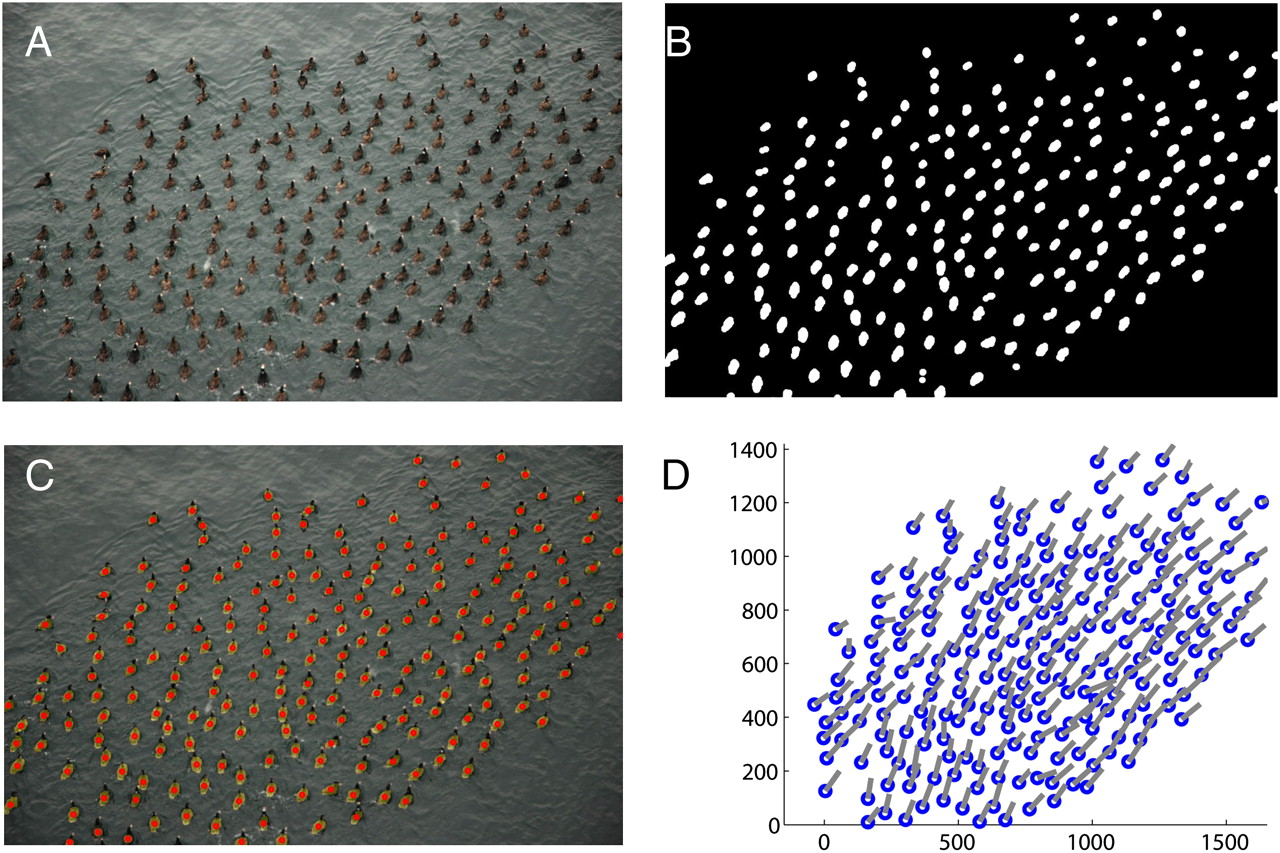
\includegraphics[width=\textwidth]{/data/thesis/fig/lukeman_data.jpg}
	\caption{Image field data and the process of transformations to extract positions of a flock of surf scoters \citep{lukeman10}.}
	\label{fig:lukeman_data}
\end{figure}

Initial work was limited to tracking small numbers of individuals in groups. In these studies individuals were not linked through frames and hence the collected data had no dynamic component. The first breakthrough came from \citet{cullen65} who used stereo photography to record the positions of fish in three dimensions. Fish are an appealing subject to study as experiments are easily conducted in a laboratory setting. Furthermore, the movements of fish can effectively be restricted to two dimensions by conducting the experiments in shallow water. Because of these benefits, further research also concentrated on fish \citep{van_long85, partridge80}. Having collected empirical data, these studies investigate properties such as the distance of individuals to their nearest neighbour, or the direction toward the nearest neighbour. Empirical studies were also made of small groups of flocking birds, with similar statistics and properties realised \citep{major78, budgey98}.

More recently, a breakthrough study by \citet{ballerini08} reconstructed the three dimensional positions of flocks of starlings consisting of up to $3,000$ individual members. The study made a static analysis of the resulting 3D dataset. Their analysis suggested that interactions are not dependent on metric distance (interactions with agents within a fixed distance), as most models in the literature assume, but on a topological distance (interaction with a fixed number of closest agents, irrespective of distance). This analysis suggested that on average a starling interacts with between six and seven of its closest neighbours. They argue that a topological interaction improved group cohesion when under attack from predation.

A significant contribution to the field was made by \citet{lukeman10}, whom collected and analysed data of large numbers of diving ducks interacting on the surface of a lake. Crucially, this dataset tracked individuals between frames and therefore allowed the reconstruction of a bird's trajectory through space and time. This data showed an increase by factor of $10$ the number of individuals which could be reliably tracked though time \citep{lukeman09}.

Analysis of empirical data has focused on properties of individuals such as nearest neighbour distances or angular neighbour densities. Research has then focused on fitting models which best replicate these properties.

\section{Numerical Studies}
\label{sec:numerical_studies}

\color{red} In which I plan to discuss the work by \citet{mann11}, and how our work extends on his. \color{black}

\section{Bayesian Statistcs}	
\label{sec:bayes_intro}

\color{red} NOTE: move this section to its own chapter. \color{black}

As part of this project we wish to infer the parameters of collective-behaviour models, given real field observations. We shall perform our statistical inference within a Bayesian framework. In this chapter we shall introduce and give overviews of some important concepts of Bayesian inference, and outline schemes we can use to infer parameters in the case of intractable likelihoods.

\subsection{Bayesian Inference}
\label{ssec:bayes}

Using Bayesian inference we wish to quantify beliefs and uncertainties about parameters $\bm{\theta} = (\theta_1, \theta_2,\dots,\theta_n)$, using data $\bm{x}$ which we observe. Given this observed data, the likelihood function for the parameters is defined
\[
    L(\bm{\theta}|\bm{x}) = f(\bm{x}|\bm{\theta}).
\]
The likelihood quantifies the probability distribution of the data in terms of the parameters. We may then specify our prior knowledge about the parameters $\bm{\theta}$ through the prior distribution $\pi(\bm{\theta})$. Bayes Theorem can then be used to incorporate both the likelihood function and our prior beliefs, to form the posterior distribution
\begin{equation}
\label{eq:bayes_theorem}
    \pi(\bm{\theta}|\bm{x}) = \frac{\pi({\bm{\theta}})L(\bm{\theta}|\bm{x})}{\int_{\bm{\theta}} \pi(\bm{\theta})L(\bm{\theta}|\bm{x})d\bm{\theta}}.
\end{equation}
Because the integral in the denominator is not a function of $\bm{\theta}$, we may consider it a constant of proportionality and express our posterior beliefs as proportional to the product of the likelihood and prior, that is
\begin{align*}
    \pi(\bm{\theta}|\bm{x}) &\propto \pi(\bm{\theta}) \times L(\bm{\theta}|\bm{x})\\
    \text{posterior} &\propto \text{prior} \times \text{likelihood}
\end{align*}

\subsection{Markov chain Monte Carlo (MCMC)}
\label{ssec:mcmc}

For the most part, the normalising constant (given in the denominator of Equation \eqref{eq:bayes_theorem}) will have multiple dimensions, not produce a density function of standard form, and be difficult to evaluate in all but the most trivial cases. Markov chain Monte Carlo algorithms provide methods to sample from the targeted density $\pi(\bm{\theta}|\bm{x})$, whilst avoiding evaluating the troublesome normalising constant.

\subsubsection{Gibbs sampling}
\label{sssec:gibbs_sampling}
One may use the full conditional distributions of parameters to sample from a multivariate density. Doing so is to implement the Gibbs algorithm. So, instead of sampling from the full posterior, we sample from the conditional posteriors of the parameters one at a time. The Gibbs algorithm is useful when the conditional densities can be expressed in standard form and are easy to sample form.

Say we wish to target the density $\pi(\bm{\theta})$ where $\theta = (\theta_1, \theta_2, \dots, \theta_p)'$, where the full conditional densities are $\pi(\theta_i|\theta_1, \theta_2, \dots, \theta_{i-1}, \theta_{i+1}, \dots, \theta_p)$, for $i=1,\dots,p$, then we may use the Gibbs sampler, as described in Algorithm \ref{alg:gibbs}.

\begin{algorithm}
\caption{Gibbs}
\label{alg:gibbs}
\begin{enumerate}
    \setcounter{enumi}{-1}
    \item Initialise chain with $\bm{\theta}^{0}$. Set $j=1$.
    \item Generate $\bm{\theta}^{j}$ from $\bm{\theta}^{j-1}$ by simulating from:
    \begin{align*}
            {\theta_1}^{j} &\sim \pi({\theta_1}^{j}|{\theta_2}^{j-1},\dots,{\theta_p}^{j-1},\bm{x})\\
            {\theta_2}^{j} &\sim \pi({\theta_2}^{j}|{\theta_1}^{j}, {\theta_3}^{j-1}, \dots, {\theta_p}^{j-1},\bm{x})\\
            &\hspace{0.25cm}\vdots \\
            {\theta_p}^{j} &\sim \pi({\theta_n}^{j}|{\theta_1}^{j}, \dots, {\theta_{p-1}}^{j-1},\bm{x})
    \end{align*}
    \item Increment $j$ to $j+1$. Repeat from step $1$.
\end{enumerate}
\end{algorithm}

\subsubsection{Metropolis-Hastings}
\label{sssec:metropolis_hastings}
The Metropolis-Hastings algorithm is another MCMC scheme. The algorithm was introduced by \cite{metropolis53}, and this work was later generalised by \cite{hastings70}. The algorithm works by constructing a Markov chain which has stationary distribution equivalent to the distribution of interest.
\begin{algorithm}
\caption{Metropolis-Hastings}
\label{alg:metropolis_hastings}
\begin{enumerate}
    \setcounter{enumi}{-1}
    \item Initialise chain with $\bm{\theta}^{0}$. Set $j=1$.
    \item Propose ${\bm{\theta}}^*$ by sampling from $q(\cdot|{\bm{\theta}}^{j-1})$, where $q$ is some proposal distribution
    \item Construct the acceptance probability $\alpha({\bm{\theta}}^*|{\bm{\theta}^{j-1}})$ as
    \begin{equation*}
		\alpha({\bm{\theta}}^*|\bm{\theta}) = \text{min}\bigg\{ 1, \frac{\pi({\bm{\theta}}^*)}{\pi({\bm{\theta}}^{j-1})} \frac{L(\bm{\theta}^*|\bm{x})}{L({\bm{\theta}}^{j-1}|\bm{x})} \frac{q({\bm{\theta}}^{j-1}|{\bm{\theta}}^*)}{q({\bm{\theta}}^*|{\bm{\theta}}^{j-1})} \bigg\}.
    \end{equation*}
    \item With probability $\alpha({\bm{\theta}}^*|{\bm{\theta}^{j-1}})$ set ${\bm{\theta}}^j = {\bm{\theta}}^*$, otherwise set ${\bm{\theta}}^j = {\bm{\theta}}^{j-1}$.
    \item Increment $j$ to $j+1$. Repeat from step $1$.
\end{enumerate}
\end{algorithm}

The algorithm begins by initialising the chain with parameters $\bm{\theta}^{0}$. Next, the algorithm proposes new values ${\bm{\theta}}^*$ from a proposal distribution, $q(\bm{\theta}^*|{\bm{\theta}}^{j-1})$, which is chosen to have the same support as the target distribution. After this, the proposed values ${\bm{\theta}}^*$ are either accepted or rejected, depending on the evaluation of the acceptance probability $\alpha({\bm{\theta}}^*|{\bm{\theta}^{j-1}})$. Because the acceptance probability depends on a ratio of $\pi(\cdot|\bm{x})$, the normalising constants cancel and therefore the target distribution only has to be known to a constant of proportionality.

\subsubsection*{Choosing a Proposal Distribution}
\label{sssec:proposal_distribution}
The practitioner must choose a suitable proposal distribution $q(\bm{\theta}^*|\bm{\theta})$. Ideally the choice of proposal distribution will give rapid convergence to $\pi(\bm{\theta}|\bm{x})$ and efficiently explore the support of $\pi(\bm{\theta}|\bm{x})$.

A special case of Metropolis-Hastings arises when the proposal distribution is symmetric, that is
\begin{equation*}
	q(\bm{\theta}^*|\bm{\theta}) = q(\bm{\theta}|\bm{\theta}^*).
\end{equation*}
In this case we get some cancellation in the acceptance ratio, and it simplifies to become 
\begin{equation*}
\alpha({\bm{\theta}}^*|\bm{\theta}) = \text{min}\bigg\{ 1, \frac{\pi({\bm{\theta}}^*)}{\pi({\bm{\theta}}^{j-1})} \frac{L(\bm{\theta}^*|\bm{x})}{L({\bm{\theta}}^{j-1}|\bm{x})} \bigg\}.
\end{equation*}

Another special case of Metropolis-Hastings is the random walk sampler. In this case one makes proposals as
\begin{equation*}
	\bm{\theta}^* = \bm{\theta}^{j-1} + \bm{\omega}^{j-1},
\end{equation*}
where the $\bm{\omega}$ are drawn from
\begin{equation*}
	\bm{\omega}^{j-1} \sim \mathcal{N}_p(\bm{0}, \Sigma).
\end{equation*}
The parameter $\Sigma$ is called the tuning parameter and controls how the chain moves around the sample space. Mixing describes how well the chain moves around the sample space and how long it takes for the chain to converge to the target distribution.

Crucially then, the parameter $\Sigma$ controls the mixing of the chain. So, naturally, we wish to choose $\Sigma$ in some optimum way, to try and improve mixing. If the target distribution is Gaussian, it has been shown that $0.234$ is an optimum acceptance probability. \citep{roberts01}. In an attempt to tune $\Sigma$ to obtain the optimum acceptance probability, a common technique is to use 
\begin{equation*}
	\Sigma = \frac{2.38^2}{2} \widehat{\text{Var}}(\bm{\theta}|\bm{x}).
\end{equation*}

\subsubsection*{Convergence Diagnostics}
\label{sssec:convergence_diagnostics}
Though there are theoretical methods to assess the convergence of chains, it is an attractive idea to analyse the output of our scheme in an attempt to assess whether the chain has converged. One of the simplest ways to assess convergence with this informal method is to inspect the trace plots of our scheme, and check for any irregularities. It is also good to use autocorrelation plots to assess autocorrelation between samples at different lags.

One way to lower autocorrelation between samples is to thin the output. When thinning, every $k$-th sample from a chain is kept, and the rest are discarded. Another common technique is to allow for a burn-in period. The purpose of a burn-in period is to discard any samples from before the chain has converged.

\subsubsection*{Blocking Parameters}
\label{sssec:blocking_parameters}
In the schemes considered so far the proposal, acceptance and rejection of the entire parameter space $\bm{\theta}$ happened simultaneously. This approach becomes inefficient for high-dimensional problems. Consider that as the dimension of the problem increases, the chances of proposing a value $\theta_i^*$ in the tails of the posterior distribution increases. Increasing the likelihood of proposing a component $\theta_i$ out in the tails of the distribution in turn decreases the acceptance rate of the chain and leads to slower convergence.

To overcome this problem the parameter space $\bm{\theta}$ can be split into blocks of parameters $\bm{\theta}_1, \bm{\theta}_2, \dots, \bm{\theta}_d$ which are proposed and accepted or rejected separately. There are no theoretical results which determine how best to block the parameter space, though typically blocks are chosen to contain related parameters.